%=================================================================
\section{Introduction}
\label{sec-intro}
In 2018, film revenue has increased significantly, and the film industry is more popular than ever.
What kind of movies make high box office receipts. In the process of preparation and shooting, 
whether the budget, the number of directors and actors have a great impact. Whether the publicity and 
preview of later films will affect the final box office income of films.

Data Analysis aims to show the relationship between attributes and box office revenue 
according to the data provided. And further integration of data, delete irrelevant data, 
unified data values and so on.

Models and Forecasts aims to use the integrated data to train the relevant models, 
improve the accuracy, and make the box office revenue forecast for some of the given data.

In this paper, we train the random forest model with the integrated data, 
and use the model to predict the box office of movies.
\section{Preliminaries} \label{sec-preliminaries}
In the early stage, the existing data were visually analyzed.

In the pre production budget, the number of actors and the number of directors and other crew members on the impact of box office.

\begin{center}
  \begin{minipage}{0.3\linewidth}
  \centering
    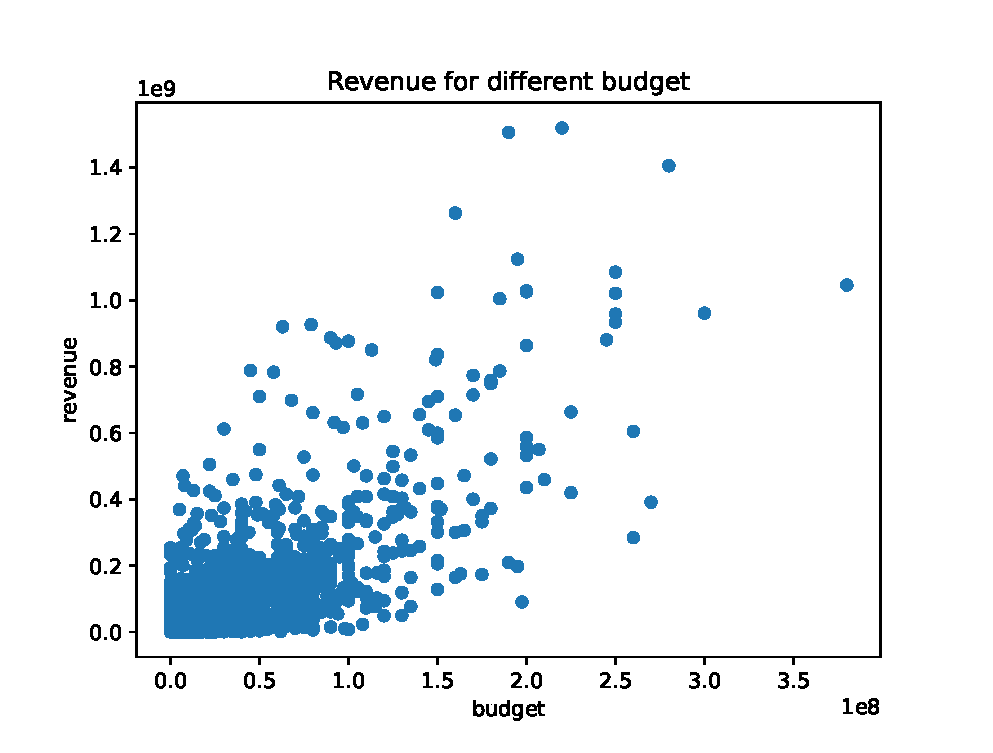
\includegraphics[width=0.8\linewidth]{figures//budget.eps}
  {\small{Budget}}
  \end{minipage}
  \hfill
  \begin{minipage}{0.3\linewidth}
  \centering
    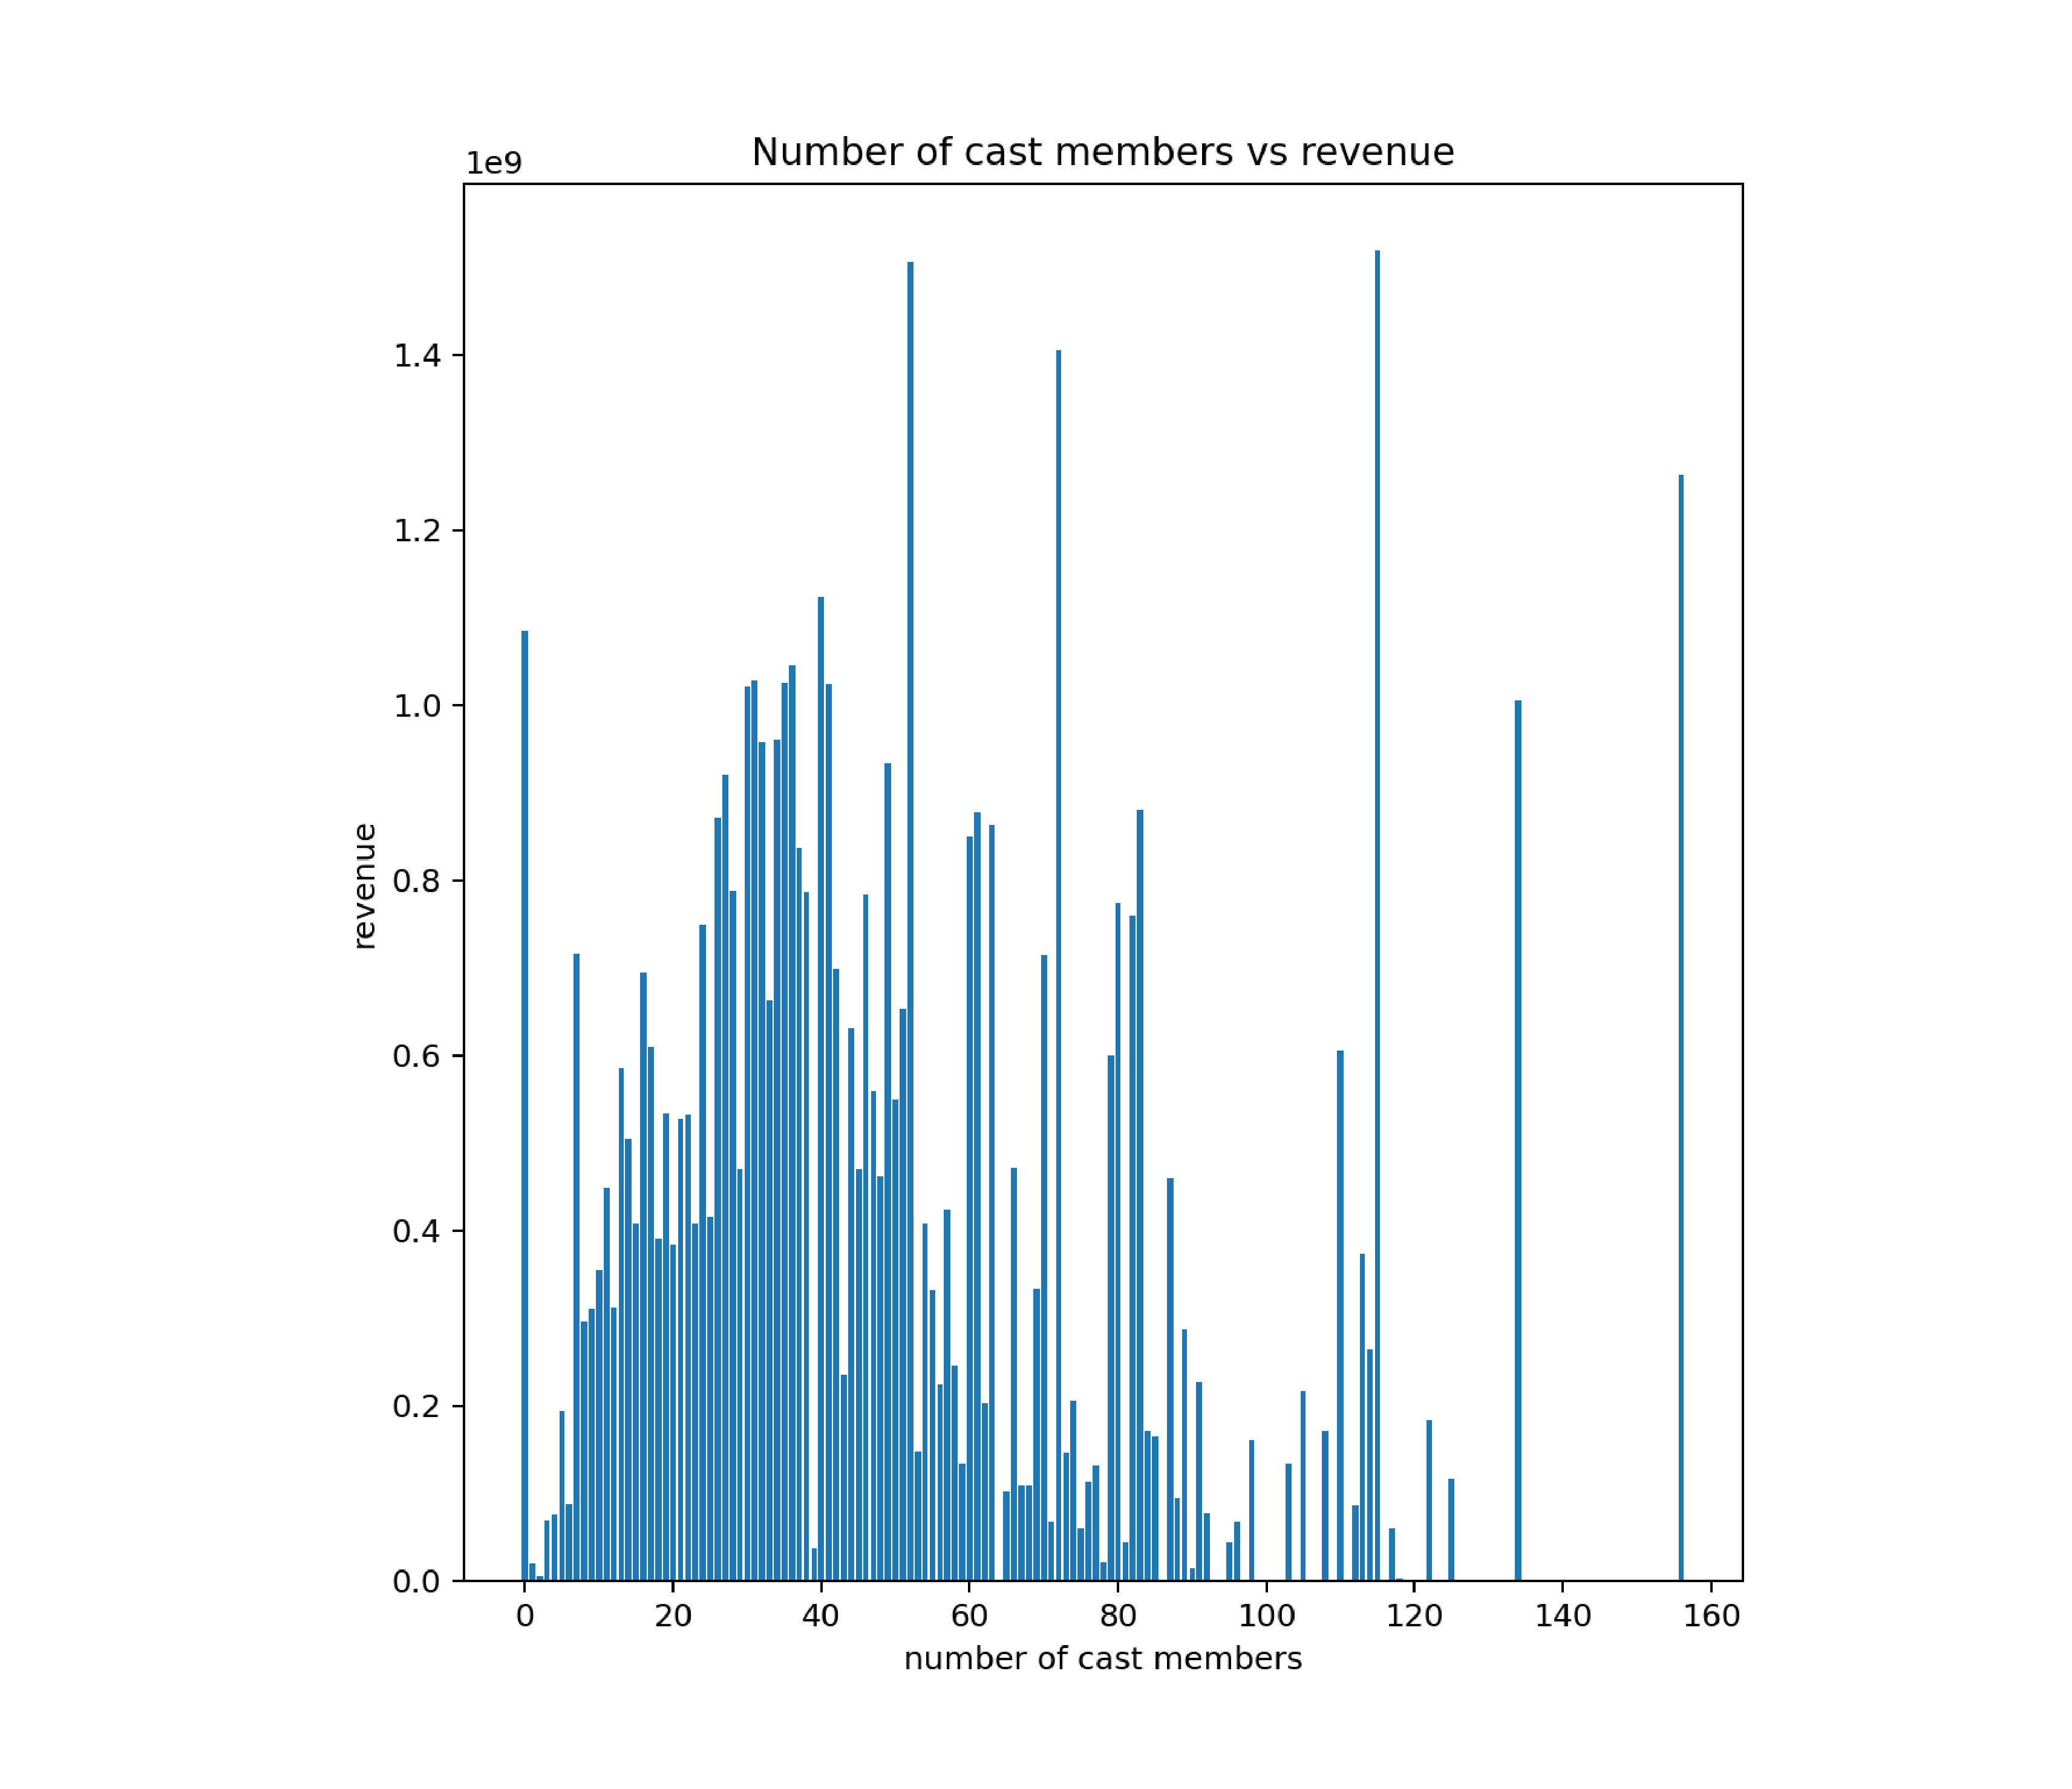
\includegraphics[width=0.8\linewidth]{figures//cest.eps}\\
  {\small{Cast}}
  \end{minipage}
  \hfill
  \begin{minipage}{0.3\linewidth}
  \centering
    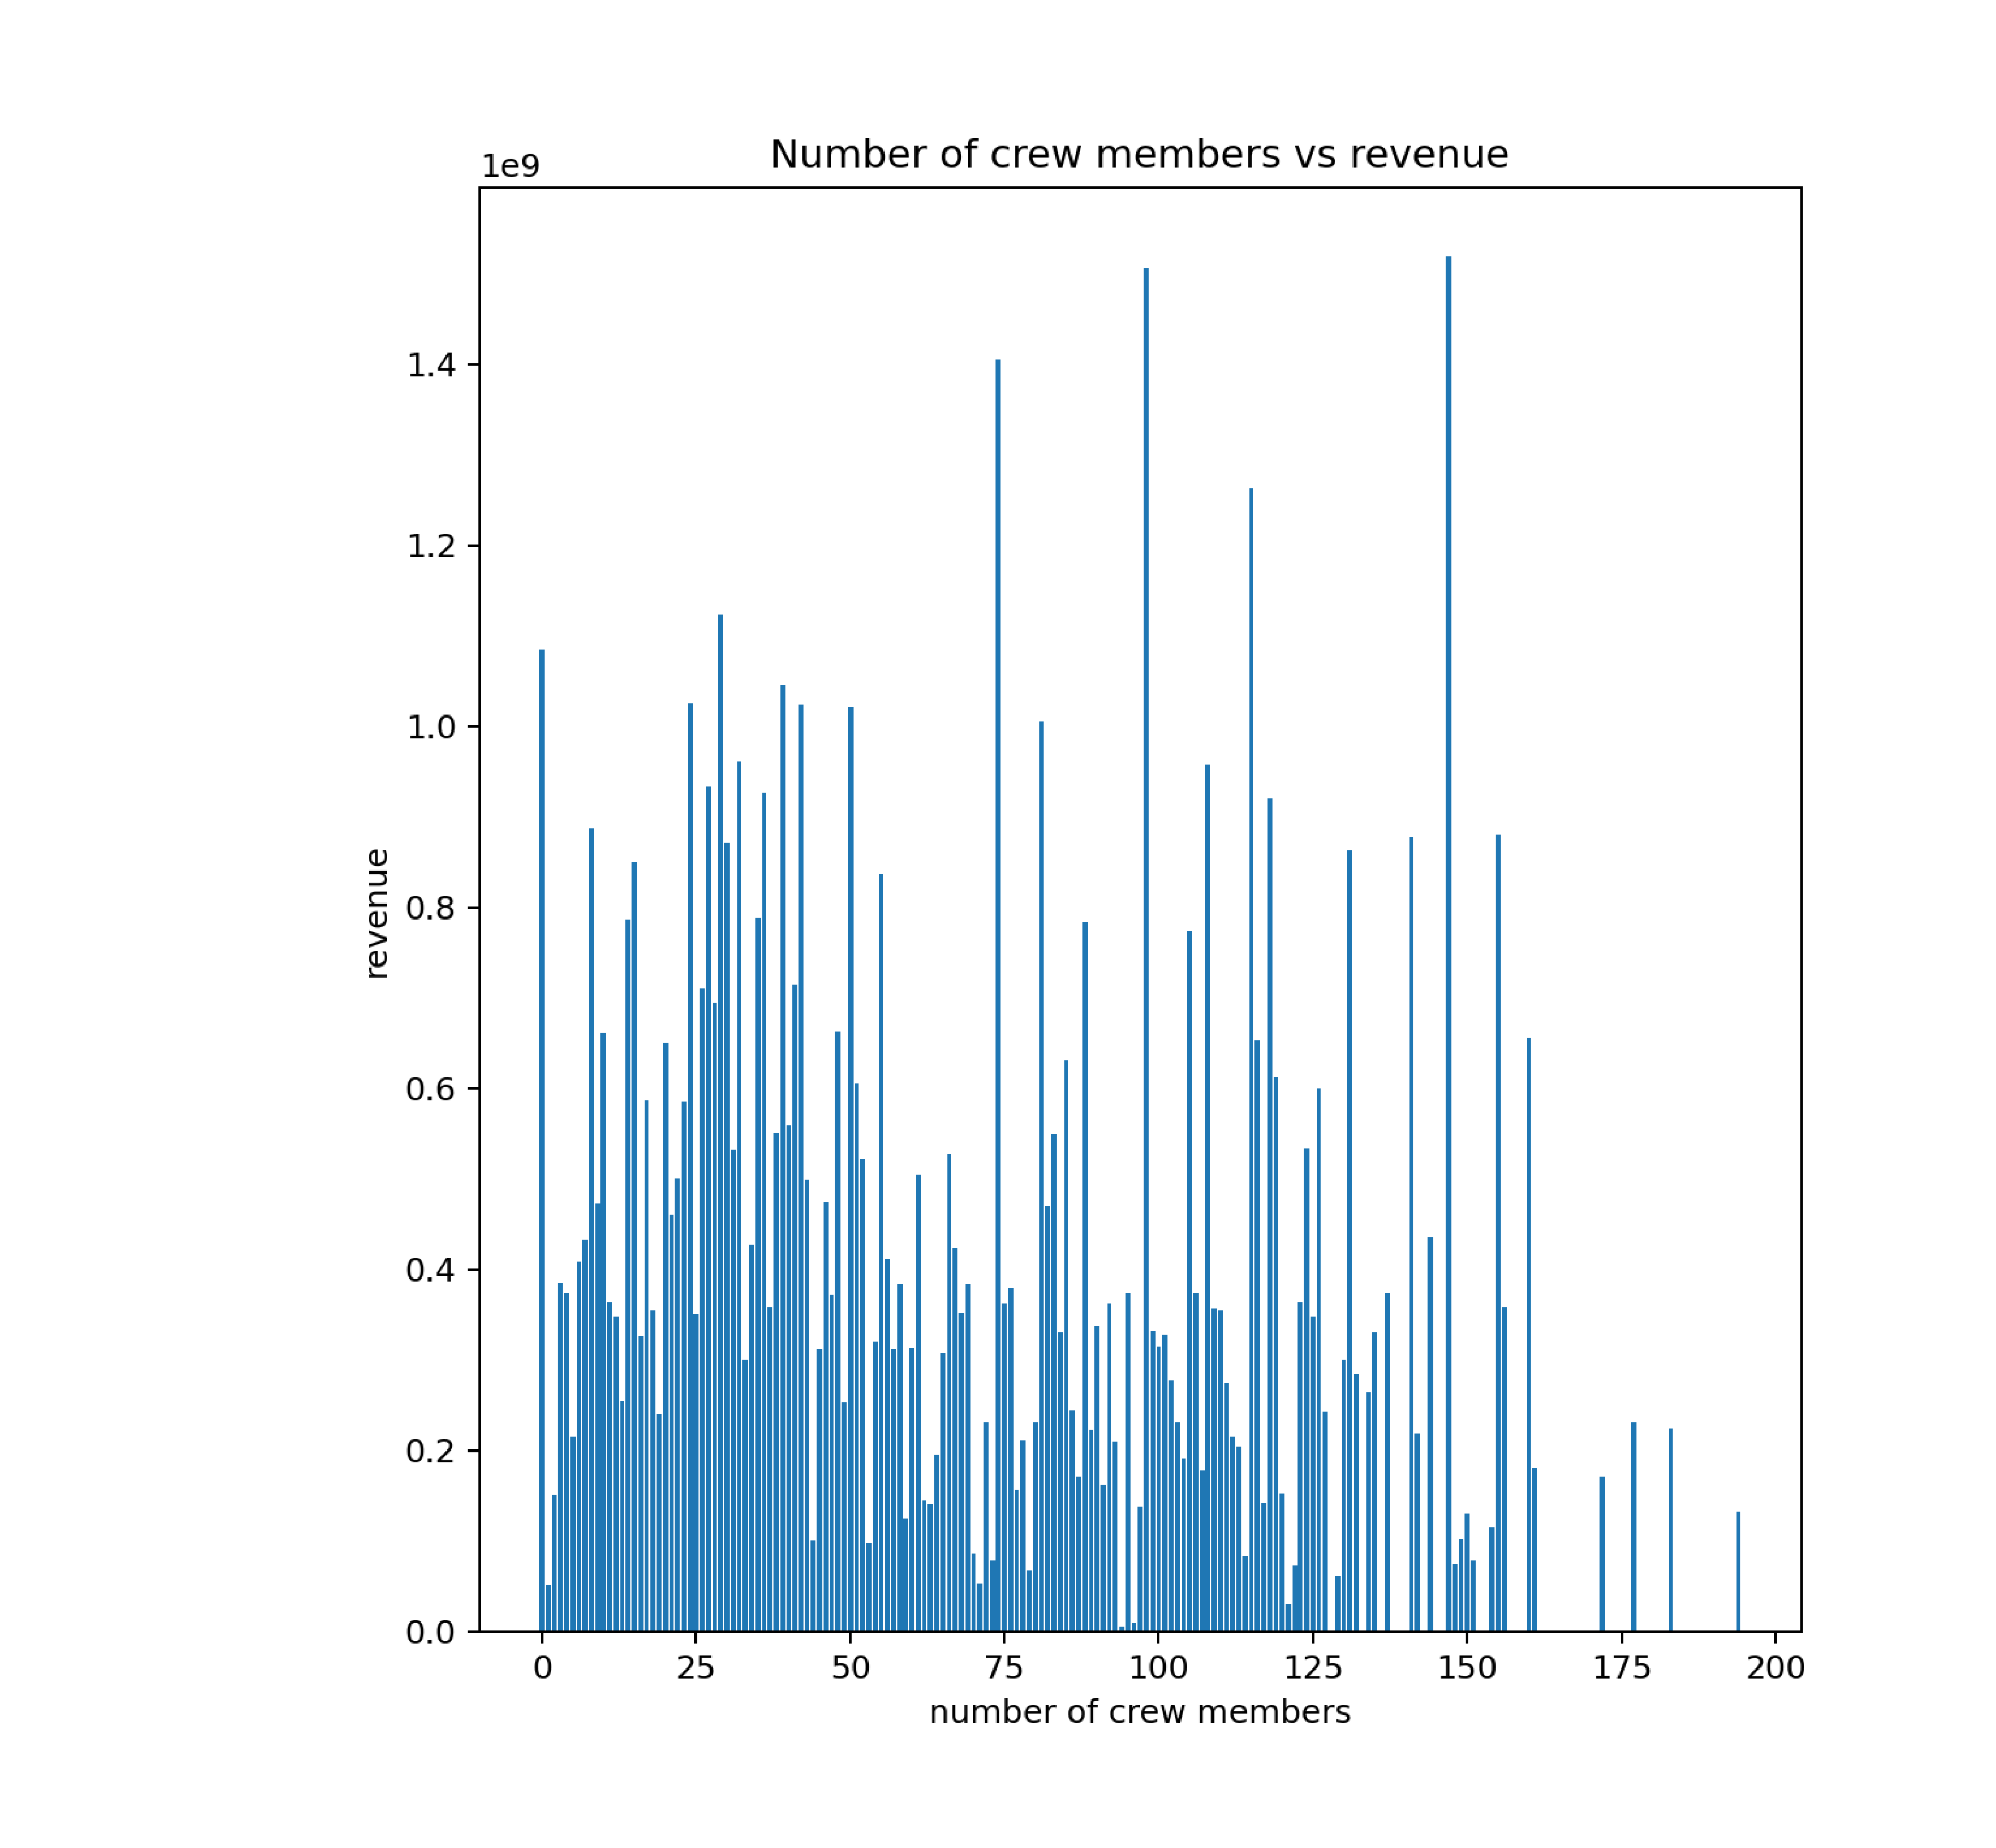
\includegraphics[width=0.8\linewidth]{figures//crew.eps}\\
  {\small{Crew}}
  \end{minipage}
\end{center}

In the late stage of film production, the influence of home page, film introduction, film tagline on the box office of films is also discussed.

\begin{center}
  \begin{minipage}{0.3\linewidth}
  \centering
    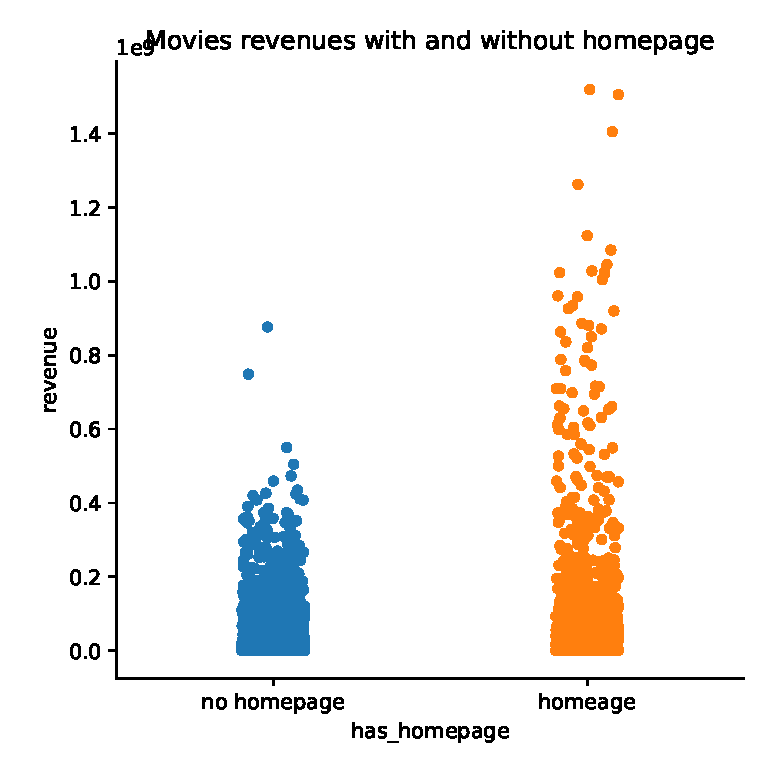
\includegraphics[width=0.8\linewidth]{figures//has_homepage.eps}
  {\small{Homepage}}
  \end{minipage}
  \hfill
  \begin{minipage}{0.3\linewidth}
  \centering
    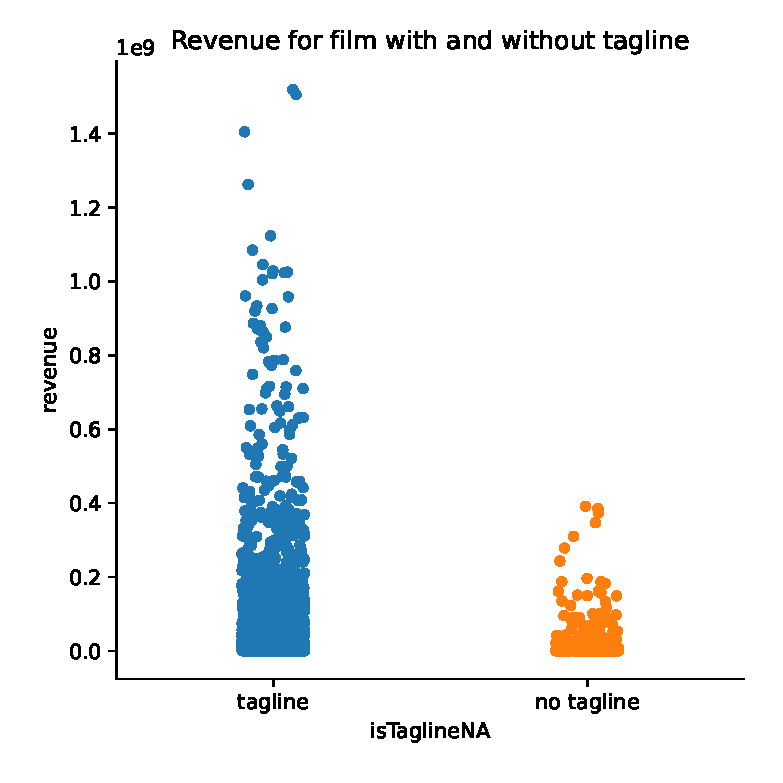
\includegraphics[width=0.8\linewidth]{figures//isTanglineNA.eps}
  {\small{Tagline}}
  \end{minipage}
  \hfill
  \begin{minipage}{0.3\linewidth}
  \centering
    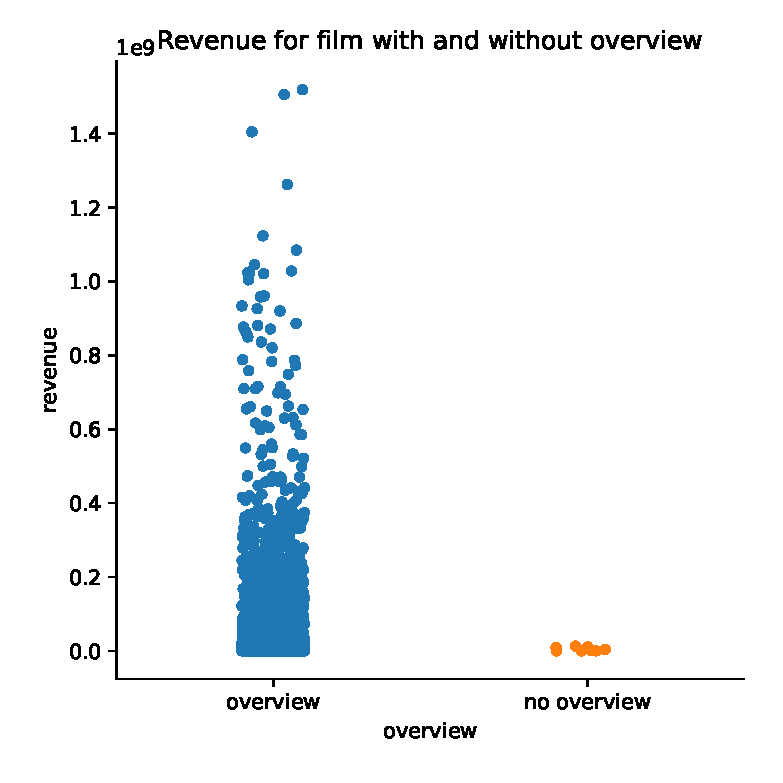
\includegraphics[width=0.8\linewidth]{figures//overview.eps}
  {\small{Overview}}
  \end{minipage}
\end{center}

Some other influences, such as film series, film companies and the number of film companies participating in the investment, etc.
\begin{center}
  \begin{minipage}{0.3\linewidth}
  \centering
    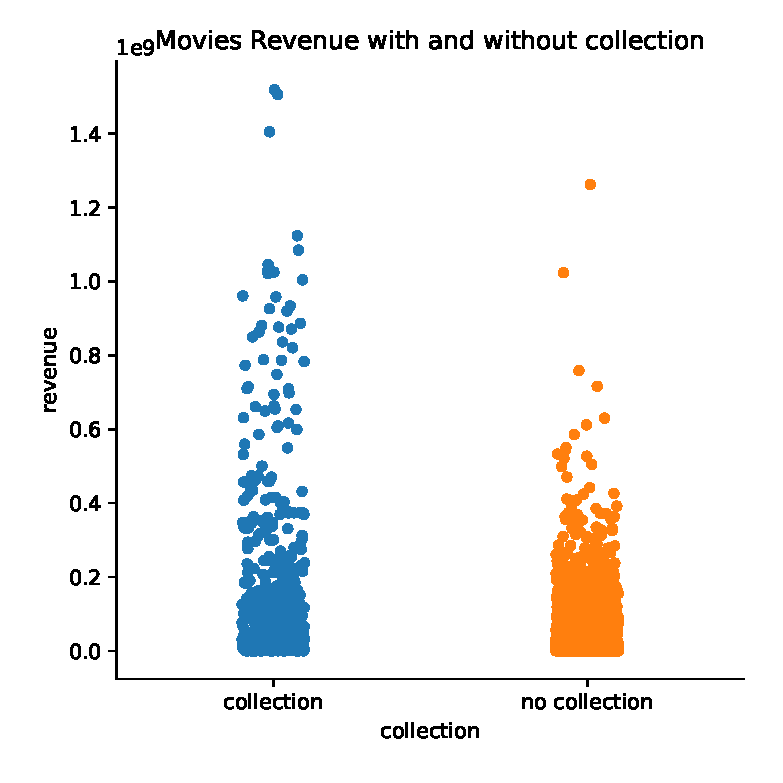
\includegraphics[width=0.8\linewidth]{figures//collection.eps}
  {\small{File Series}}
  \end{minipage}
  \hfill
  \begin{minipage}{0.3\linewidth}
  \centering
    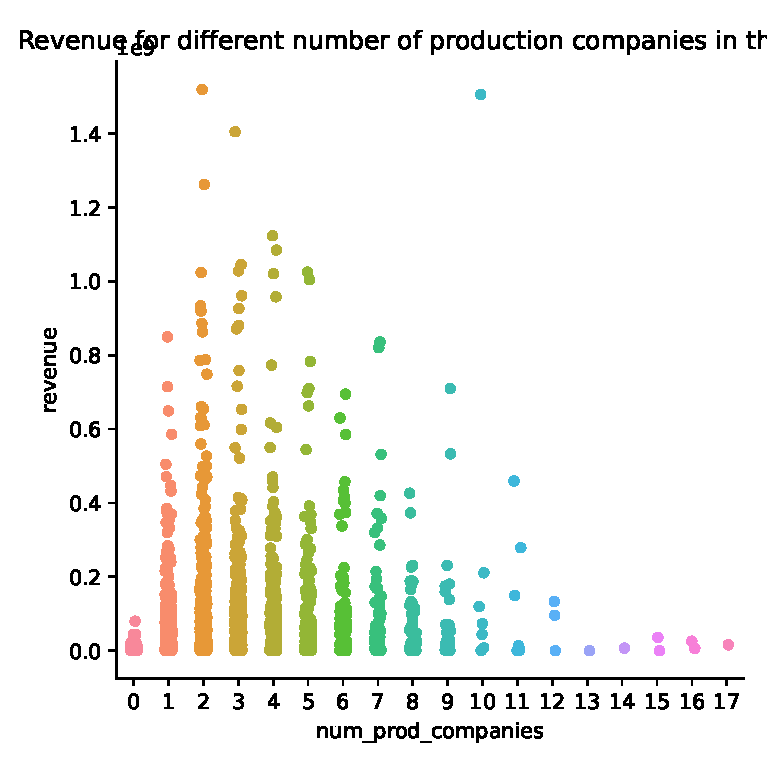
\includegraphics[width=0.8\linewidth]{figures//company.eps}
  {\small{File Company}}
  \end{minipage}
  \hfill
  \begin{minipage}{0.3\linewidth}
  \centering
    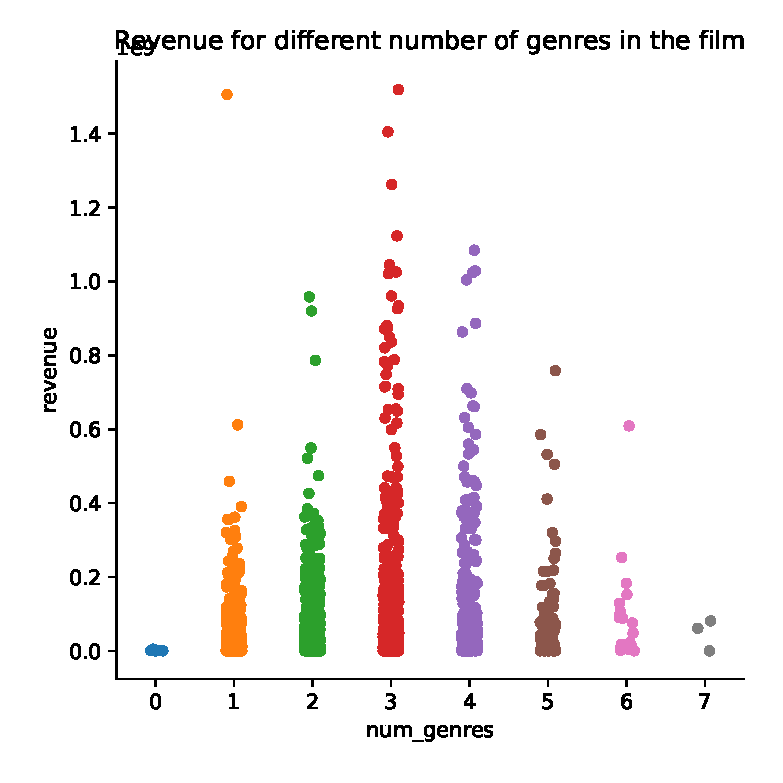
\includegraphics[width=0.8\linewidth]{figures//counrty.eps}
  {\small{Company Number}}
  \end{minipage}
\end{center}

The popularity of the film's language and genre among the audience also affects the box office.

\begin{center}
  \begin{minipage}{0.4\linewidth}
  \centering
    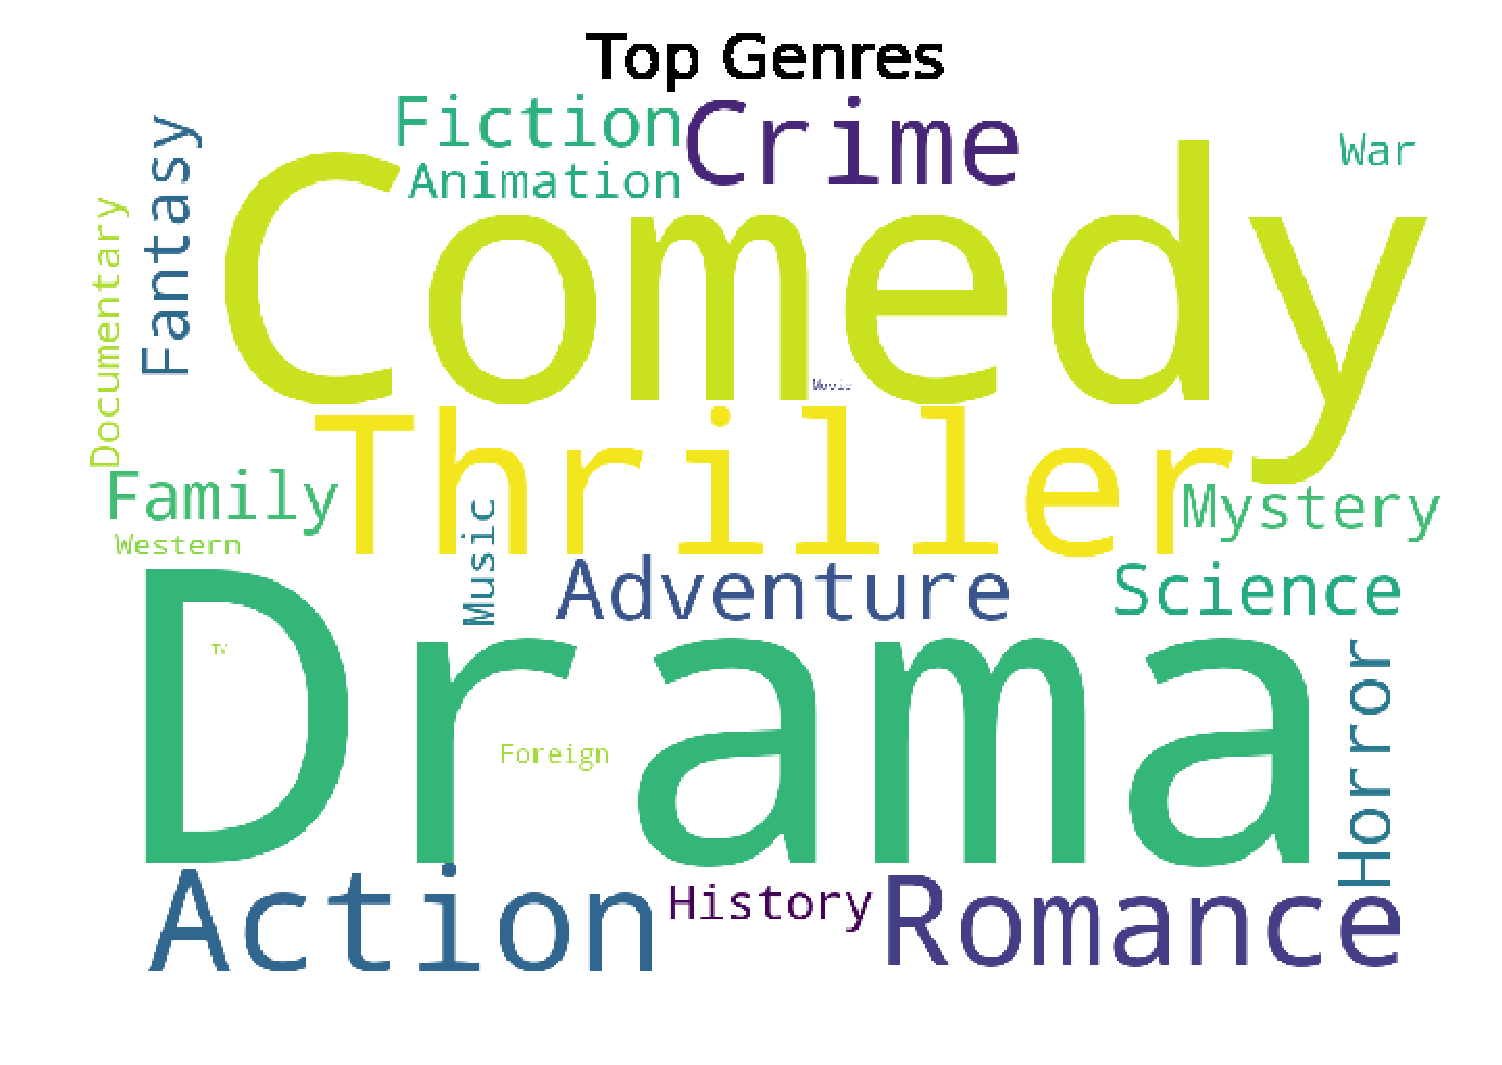
\includegraphics[width=0.8\linewidth]{figures//genre_clold.eps}\\
  {\small{Genre}}
  \end{minipage}
  \hfill
  \begin{minipage}{0.4\linewidth}
  \centering
    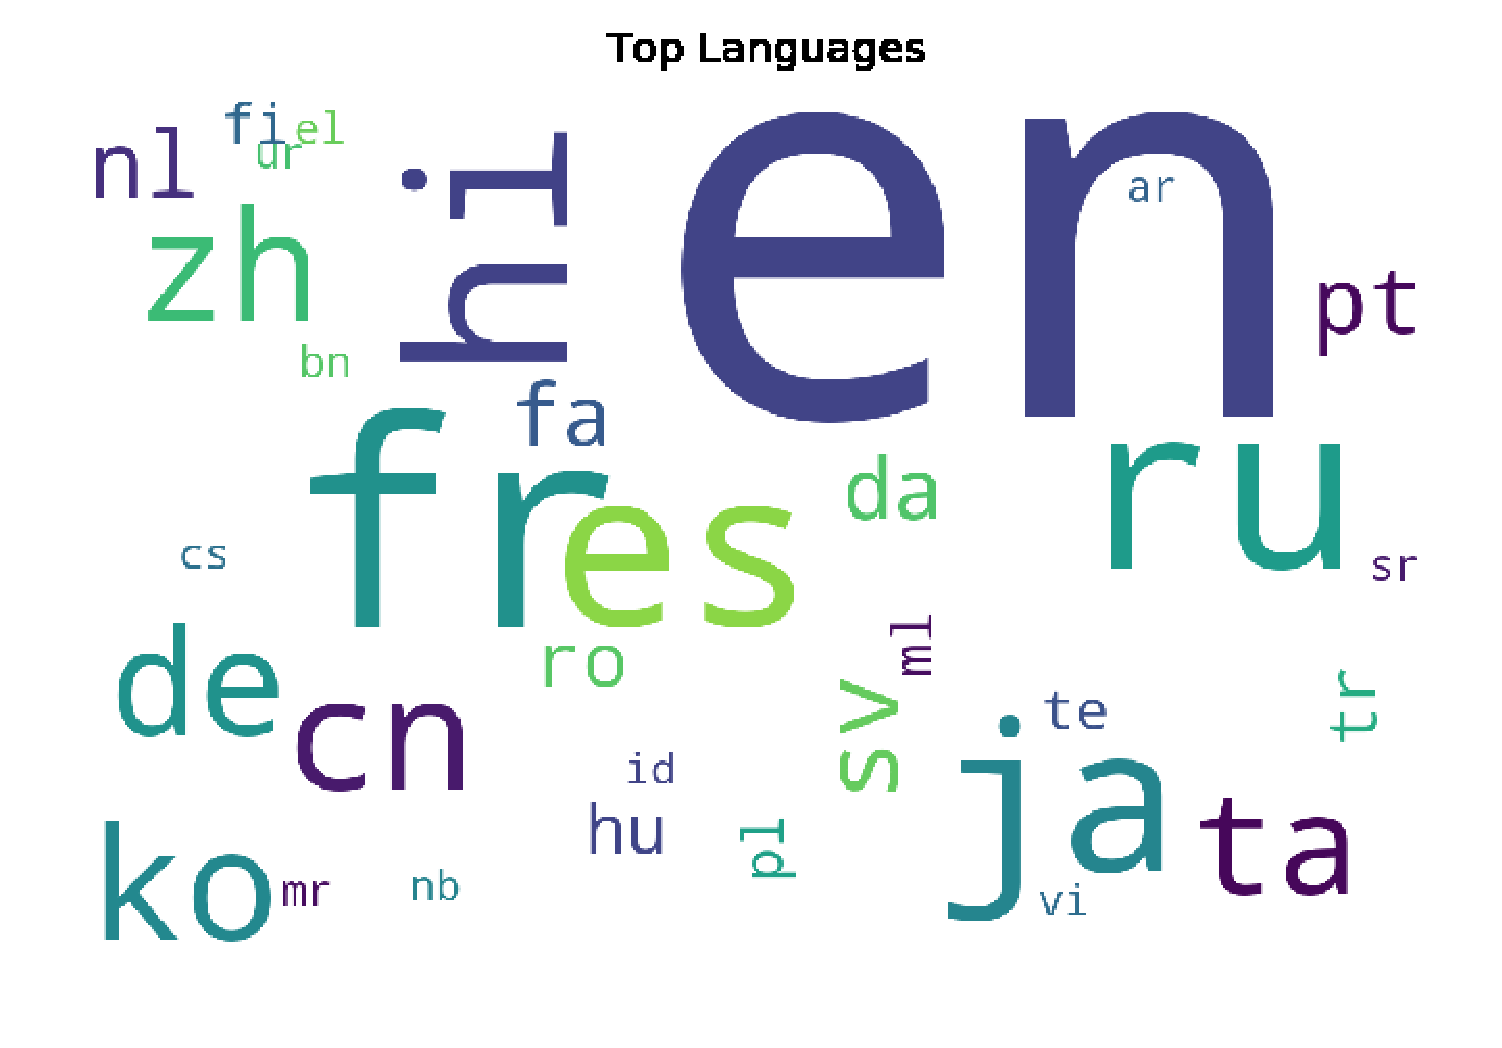
\includegraphics[width=0.8\linewidth]{figures//language.eps}\\
  {\small{Language}}
  \end{minipage}
  \hfill
\end{center}

\section{Method} \label{sec-method}
After the preparatory work, the data are further processed.

Processing data that does not affect the box office.

%5\begin{table}
%  \begin{center}
%    \centering
%    \caption{Partial Processing Data}
%    \begin{tabular}{ c | c }
%      \toprule
%      Name     &  Description        \\
%      \midrule
%      imdb id       &  ID of movie in TMDB  \\
%      orginal title &  The original name of the movie \\
%      poster path &  Movie poster link \\
%      status   & The state of the film \\
%      keywords      &  Key words of movies \\
%      tagline &  The slogan of the film \\
%      homepage & Official film Homepage \\
%      overview   &A brief description of the film \\
%      collection & Series name of film series\\
%      release date & Film release time\\ 
%      \bottomrule
%      \end{tabular}
%  \end{center}
%\end{table}

Normalization of training data and test data.


After the completion of data processing, the model was established using random forest algorithm.

Random Forest Algorithm is an ensemble technique that combines multiple decision trees. 
    Other advantages of random forests are that they are less sensitive to outliers in the dataset 
    and don’t require much parameter tuning.

%\section{Experiment} \label{sec-experiment}
%After the training of the model, the prediction was made by using the data.

\section{Conclusions} \label{sec-conclusions}
The investment in the early stage and publicity in the later stage have an impact on the box office.

In the early stage, the number of actors and crew should be moderate, not the more the better.

The prediction accuracy can be further improved, such as using XGBoost.
\section*{Acknowledgment}

Thanks for the learning opportunities provided by Tulip, 
I grew up rapidly in this period of time. 
Thanks to my tutor for answering questions and puzzles during my study, 
which is my rapid progress. At the same time, I should also like to thank my senior brother, 
sister and classmates for their help. When I am not successful in my study, 
I will lend a helping hand to help me solve problems.